\subsubsection{KYMCO Agility Carry 125}

\paragraph{Descripción general} 
%%El ciclomotor KYMCO Aility Carry 125 es una scooter especializado para el reparto y que además cuenta con unos niveles de emisiones mínimos. Diseñado para dar una respuesta práctica ante cualquier demanda, por lo que tiene dos amplias y robustas parrillas con capacidad de 5Kg de carga para la delantera y hasta 20Kg de carga en la trasera.
Estudiando las consideraciones descritas en \refanexo{anexo_scooter_gasolina}, se ha optado de entre todos los modelos mostrados por la KYMCO Agility Carry 125 en la \autoref{fig:KYMCO Agility Carry 125}. 

\begin{figure}[h]
    \centering
    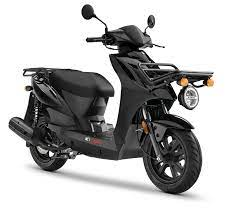
\includegraphics[scale = 0.8]{archivos/KYMCO Agility Carry 125.jpg}
    \caption{KYMCO Agility Carry 125.}
    \label{fig:KYMCO Agility Carry 125}
\end{figure}

Los motivos para elegir este modelo están basados en su especialidad para el reparto y la robustez para este tipo de tareas. La motocicleta es de una cilindrada de 125 \glssymbol{cc}, cuenta con unos niveles de emisiones mínimos y con unas parrillas delantera y trasera con capacidad de carga de hasta 5 \glssymbol{kg} y 20 \glssymbol{kg} respectivamente. Su precio actual en el mercado es de 2.149 \glssymbol{euro}.

La KYMCO Agility Carry 125 cuenta con una autonomía de 250 \glssymbol{km} debido a su depósito con capacidad de 6,5 \glssymbol{litros} y su motor de cuatro tiempos que hace que sea más eficiente. Esta autonomía es más que suficiente para realizar varias jornadas de trabajo sin repostar.

Cuenta con frenos de disco traseros y delanteros para una mayor seguridad, así como suspensiones hidráulicas para una mayor estabilidad, neumáticos de 12 pulgadas para una gran agilidad por ciudad, faros LED y un peso de tan solo 123 \glssymbol{kg}.

%El Barto

% \paragraph{Estudio del reparto.}

%  %Escoger modelo
\paragraph{Mantenimiento y robustez.}
%%Se trata de un modelo muy robusto ya que está concebido para realizar largas jornadas de trabajo.En cuanto al mantenimiento, como cualquier otra motocicleta de 125cc necesita el mantenimiento especificado en el "ANEXO X"(tabla con costes de mantenimiento).

Al ser un modelo muy robusto y concebido para realizar largas jornadas de trabajo, no tendrá tantas averías como otro modelo de motocicleta no especializada, reduciendo los costes en este aspecto.

Una motocicleta necesita mantenimiento en sus frenos, transmisión, ruedas, así como cambios de aceite y revisiones. Esto se estudia en \refanexo{anexo_precio_taller_combustible}, obteniéndose un importe anual de mantenimiento de 239 \glssymbol{euro}.
\paragraph{Viabilidad económica}
%%El coste del primer año de esta motocicleta es de 4.412,42€ y de 2.263,42€ los años sucesivos  según lo calculado en el "ANEXO X".
Para ver si es viable el gasto hay que observar el gasto fijo que supone la adquisición del equipo al completo, y posteriormente el gasto anual entre mantenimiento, seguros y combustible.

Todos los cálculos y estimaciones referentes a la viabilidad económica se pueden encontrar en la \autoref{tab:Presupuesto motocicletas de gasolina}, \refanexo{sub_anexo_calculos_motocicleta}, donde se muestran los presupuestos para ambos modelos de reparto estudiados en el estudio del reparto.

En el primer año, se han de tener en consideración el precio de mercado por unidad de las motocicletas y el número total que se van a comprar, incluyendo también el impuesto de matriculación por cada vehículo adquirido que en este modelo es de 99,77 \glssymbol{euro}. Además de esto, hay que añadir como gasto fijo inicial la adquisición del equipamiento, los cuales se enumeran en la \autoref{consideraciones_preliminares}, considerando en cada caso el número
de personal, o vehículos simultáneos en carretera.

Para los gastos anuales se debe comenzar con el coste del combustible del vehículo y el impuesto de circulación de 8,55 \glssymbol{euro}. Teniendo el precio de la gasolina, obtenido en el \refanexo{anexo_precio_taller_combustible}, se obtiene el gasto semanal y anual relacionado con el combustible. 

Los gastos relacionados con reparaciones o mantenimiento se han fijado en el \refanexo{anexo_precio_taller_combustible}, por lo que se asume un gasto mensual a cada uno.
El coste por seguro fijado es de 265 \glssymbol{euro}, lo cual se multiplicará directamente por el número de vehículos en posesión de manera mensual.

Teniendo todas las consideraciones anteriores descritas, se concluye finalmente el presupuesto necesario en el primer año y posteriores, siendo:

\begin{itemize}
    \item Presupuesto para el primer año del modelo de estudio 1 - 18.058,14 \gls{euro}
    \item Presupuesto anual del modelo de estudio 1 - 5.861,39 \gls{euro}
    \item Presupuesto para el primer año del modelo de estudio 2 - 17.591,70 \gls{euro}
    \item Presupuesto anual del modelo de estudio 2 - 5.394,95 \gls{euro}
\end{itemize}
%%Observando los resultados en \refanexo{anexo_scooter_gasolina}, \refanexo{anexo_precio_taller_combustible} y \autoref{consideraciones_preliminares_seguro} en los que se estudian detalladamente todos los costes que conlleva esta motocicleta se llega a un resultado final de que el coste que implica es de 2.149,00 \glssymbol{euro} de inversión inicial para la compra de la motocicleta y de 2.848,42\glssymbol{euro} anuales en gastos.
\paragraph{Conclusiones modelo.}
%%Es una motocicleta especializada por lo que está garantizado el perfecto cumplimiento de la tarea a realizar y una opción a considerar si no se quiere optar por los vehículos electricos.

Analizando los datos anteriores se concluye que dicha motocicleta es una opción con una gran fiabilidad, desempeño en su tarea y la opción más viable para cubrir largas distancias sin interrupción ni complicaciones. Todo esto a cambio de una mayor inversión inicial y mayor coste anual.

De las opciones que se plantean es el vehículo más seguro y que alcanza la mayor velocidad, por lo que puede realizar un mayor número de repartos, necesitando por ello menos cantidad de ellas. Dada su clasificación L3 dentro de los vehículos puede circular por autovías y autopistas en caso de que sea necesario, facilitando la labor de reparto.

Como principales inconvenientes nos encontramos con que al ser un modelo de combustión conlleva contaminación asociada, tanto medioambiental como en términos de ruido. A diferencia de las opciones eléctricas, el combustible tiene mayor coste que la energía.